\begin{ex}
(Ufrs) Cada cartela de uma coleção é formada por seis quadrados coloridos, justapostos como indica a figura abaixo:
   \begin{center}
       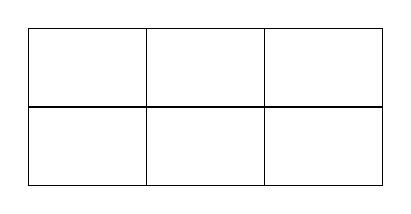
\begin{tikzpicture}
       \draw (0,0)--(4.5,0)--(4.5,2)--(0,2)--(0,0);
       \draw (0,1)--(4.5,1);
       \draw (1.5,0)--(1.5,2);
       \draw (3,0)--(3,2);
       
       \end{tikzpicture}
   \end{center}
Em cada cartela, dois quadrados foram coloridos de azul, dois de verde e dois de rosa. A coleção apresenta todas as possibilidades de distribuição dessas cores nas cartelas nas condições citadas e não existem cartelas com a mesma distribuição de cores. Retirando-se ao acaso uma cartela da coleção, a probabilidade de que somente uma coluna apresente os quadrados da mesma cor é de:
   \begin{enumerate}[(a)]
   \item 6\%
   \item 36\%
   \item 40\%
   \item 48\%
   \item 90\%
   \end{enumerate}
    \begin{sol}
     resposta: c \\
     espaço amostral: $\frac{6!}{2!\cdot21\cdot2!}=$90 \\ somente uma  coluna deve ter  quadrados da mesma cor. 
     Por exemplo: a primeira coluna com a cor V. \\
     VAR.....VAA.....VRR.....VRA\\
     VRA.....VRR.....VAA.....VAR\\
     temos 4 formas diferentes de pintura. Como são 3 colunas então temos $4\times3=12$ maneiras. Como são 3 cores temos $12\times3=36 \Longrightarrow p=\frac{36}{90}=\frac{4}{10}=40\%$
    \end{sol}
\end{ex}